\documentclass[UTF8]{ctexart}
\usepackage{xecjk}
\usepackage{fontspec}
\usepackage{metalogo}
\usepackage{amsmath}
\usepackage{newtxtt, newtxmath}

\setmainfont{Times New Roman} %英文字体CCBackBeat
\setCJKmainfont{SimSun} % 中文字体

\title{论文测试}
\author{Teemo}
\date{2019年2月22日}
\begin{document}
\maketitle
\tableofcontents
\section{输出测试}
 Hello \XeLaTeX.
 Body of the article.
 second not sure \\
 fuck LaTex \\
 换行试试?\LaTeX,WithTab Icon,How to add a command \\

 换行
\section{字体测试}
 列出如下测试
 \subsection{中文字体}
     fuck you here,latex.
     {\songti   这是宋体的样式} \par
     {\heiti    这是黑体的样式} \par
     {\fangsong 这是仿宋的样式} \par
     {\kaishu   这是楷书的样式} \par
     {\lishu   这是隶书的样式} \par
     {\youyuan 这是幼圆的样式} \par
 \subsection{英文字体}
     cao ni ma, latex.
     失败,操你妈\\
     {\font\rm="CCBackBeat" \rm This is Supercell-Magic\\}
     {\font\rm="Supercell-Magic" \rm This is <Supercell-Magic>\\}
     {\font\rm="CCBackBeat" \rm Stephen Robert Irwin (22 February 1962 – 4 September 2006),
     nicknamed "The Crocodile Hunter" was an Australian zookeeper, conservationist, and
     television personality. Irwin achieved worldwide fame from the television series The
     Crocodile Hunter (1996–2007), an internationally broadcast wildlife documentary series
     which he co-hosted with his wife Terri; the couple also hosted the series Croc Files
     (1999–2001), The Crocodile Hunter Diaries (2002–2006), and New Breed Vets (2005).
     They also owned and operated Australia Zoo, founded by Irwin's parents in Beerwah,
     about 80 kilometres (50 mi) north of the Queensland state capital city of Brisbane.}\\
     % {\supercell This is <Supercell>}

\section{章节段落}
 中国在East Asia.
 \subsection{Hello Beijing}
     北京是capital of China.
     \subsubsection{Hello Dongcheng District}
         \paragraph{Tian'anmen Square}
             is in the center of Beijing
             \subparagraph{Chairman Mao}
                 is in the center of 天安门广场。
 \subsection{Hello 山东}
     \paragraph{山东大学} is one of the best university in 山东。
         傻逼
\section{数学公式}
 \subsection{数学模式}
     LaTeX 的数学模式有两种:行内模式 (inline) 和行间模式 (display)。前者在正文的行文中,插入数学公式;后者独立排列单独成行,并自动居中。
     \subsubsection{行内模式}
         在行文中,使用 $ x^2+y^2 $ 可以插入行内公式
     \subsubsection{行间模式}
         第一段话 $ \frac{1}{2} $
         \[1+2=3\]
         第二段话
         \begin{align}
             \sqrt{\frac{n_1!}{K!(n_2-k)!}} \\
             f(x) & = (x+a)(x+b)            \\
                  & = x^2 + (a+b)x + ab     \\
             E=mc^2                         \\
             \frac{1}{2}
         \end{align}
         \[Z=r\cdot e^{2\pi i}.\]
 \subsection{符号}
 \subsection{运算符}
     \begin{align}
         \sum_{i=1}^n i \quad \prod_{i=1}^n                      \\
         \sum\limits_{i=1}^n i \quad \prod\limits_{i=1}^n        \\
         \lim_{x\to0}x^2 \quad \int_a^b x^2 dx                   \\
         \lim\nolimits_{x\to0}x^2 \quad \int\nolimits_a^b x^2 dx \\
         \int\quad \iint \quad \iiint \quad \iiiint \quad \idotsint_x^y x^{e^{2\pi^2}} dx
     \end{align}
     \subsubsection{定界符(括号)}
         %  \[ \Biggl(\biggl(\Bigl(\bigl((x)\bigr)\Bigr)\biggr)\Biggr) \]
         %  \[ \Biggl[\biggl[\Bigl[\bigl[[x]\bigr]\Bigr]\biggr]\Biggr] \]
         %  \[ \Biggl \{\biggl \{\Bigl \{\bigl \{\{x\}\bigr \}\Bigr \}\biggr \}\Biggr\} \]
         %  \[ \Biggl\langle\biggl\langle\Bigl\langle\bigl\langle\langle x
         %      \rangle\bigr\rangle\Bigr\rangle\biggr\rangle\Biggr\rangle \]
         %  \[ \Biggl\lvert\biggl\lvert\Bigl\lvert\bigl\lvert\lvert x
         %      \rvert\bigr\rvert\Bigr\rvert\biggr\rvert\Biggr\rvert \]
         %  \[ \Biggl\lVert\biggl\lVert\Bigl\lVert\bigl\lVert\lVert x
         %      \rVert\bigr\rVert\Bigr\rVert\biggr\rVert\Biggr\rVert \]
     \subsubsection{省略号}
         \[ x_1,x_2,\dots ,x_n\quad 1,2,\cdots ,n\quad
             \vdots\quad \ddots \]
 \subsection{矩阵}
     \[ \begin{pmatrix}
             a & b \\c&d
         \end{pmatrix} \\
         \begin{bmatrix}
             a & b \\c&d
         \end{bmatrix} \\
         \begin{Bmatrix}
             a & b \\c&d
         \end{Bmatrix} \\
         \begin{vmatrix}
             a & b \\c&d
         \end{vmatrix} \\
         \begin{Vmatrix}
             a & b \\c&d
         \end{Vmatrix}
     \]
     \[ \begin{pmatrix}
             a_{1,1} & a_{1,2} \cdots a_{1,n}          \\
             a_{2,1} & a_{2,2} \cdots a_{2,n}          \\
             \vdots  & \ddots                 & \vdots \\
             a_{n,1} & a_{n,2} \cdots a_{n,n}          \\
         \end{pmatrix}
     \]
     Marry has a 行内 matrix $ ( \begin{smallmatrix} a&b\\c&d \end{smallmatrix} ) $.
 \subsection{分段函数}
     \[ y= \begin{cases}
             -x,\quad x\leq 0 \\
             x,\quad x>0
         \end{cases} \]
 \subsection{插入图片和表格}
     \subsubsection{图片}
         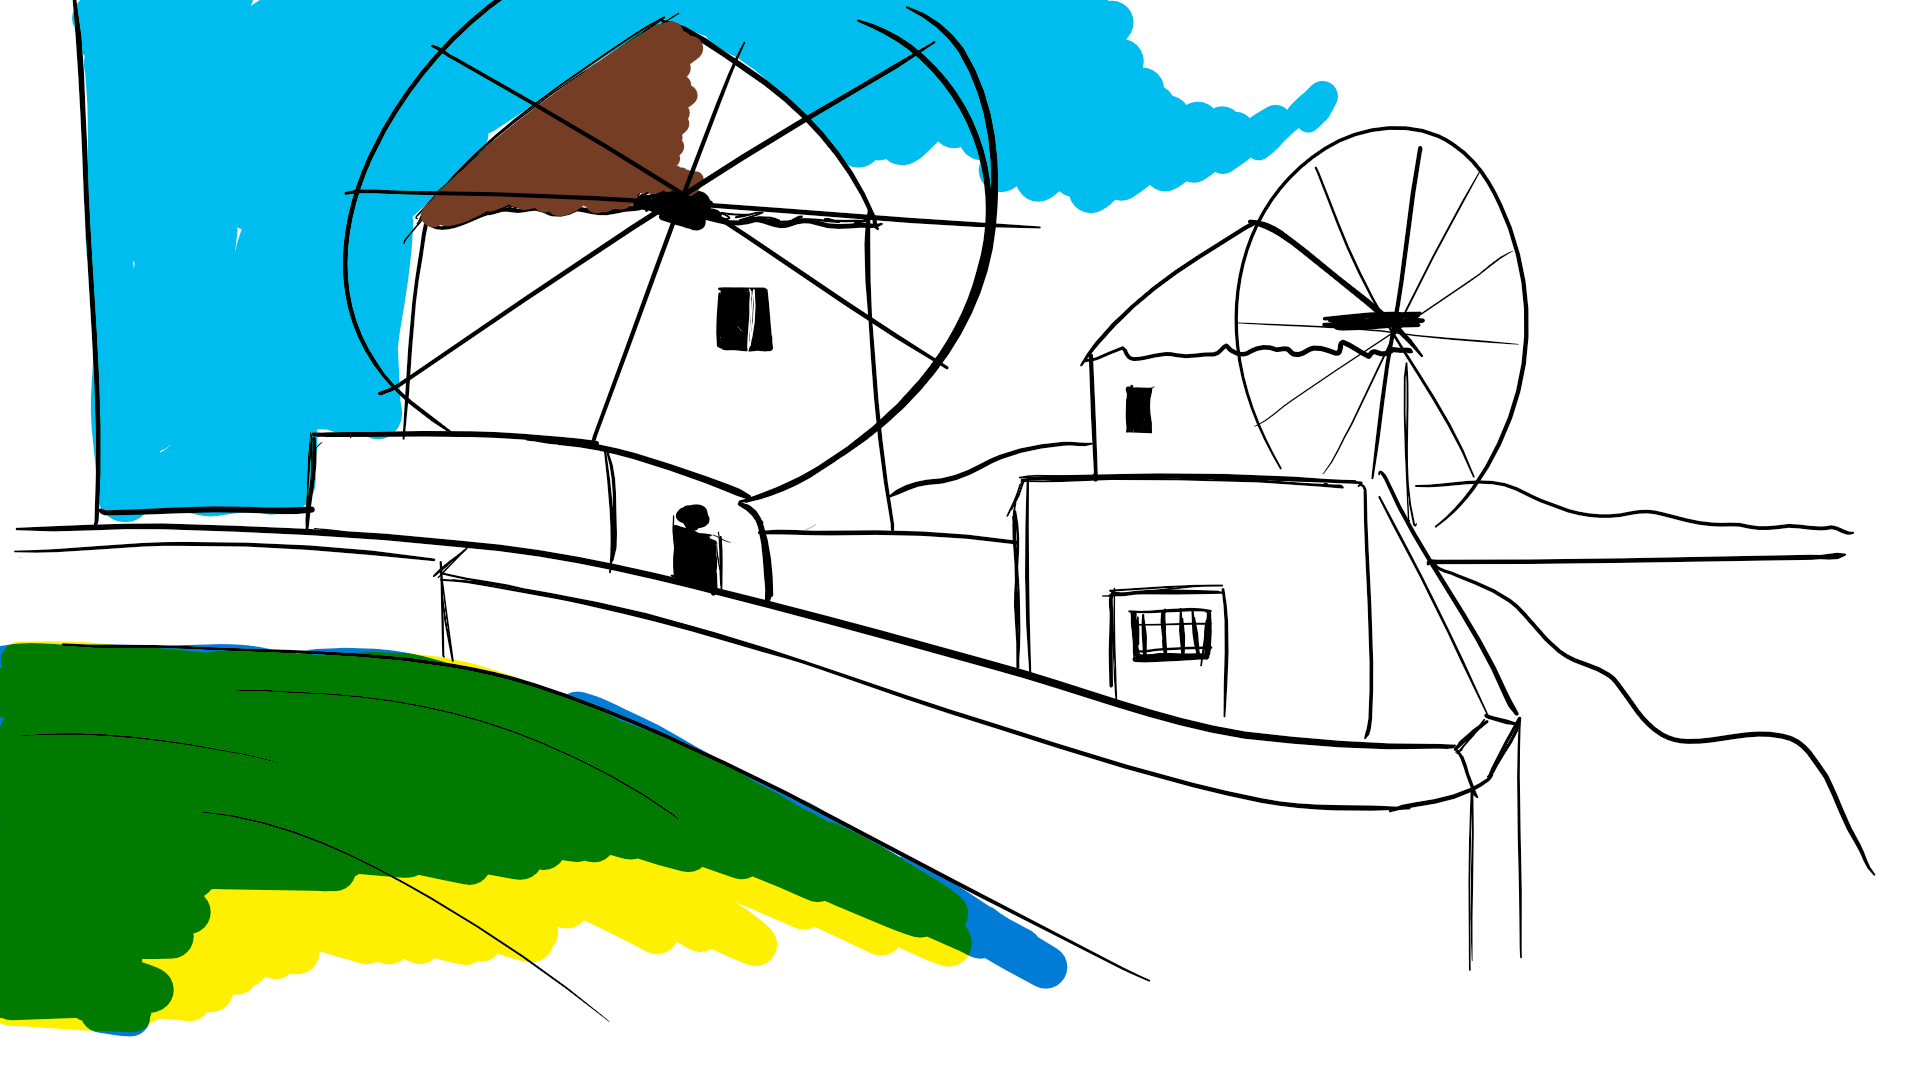
\includegraphics[width = .8\textwidth]{草图.png}
 \subsection{表格}
     tabular 环境提供了最简单的表格功能。
     它用 "hline" 命令表示横线,在列格式中用 | 表示竖线;
     用 “与” 来分列;每列可以采用居左、居中、居右等横向对齐方式,
     分别用 l、c、r 来表示。\\
     \begin{tabular}{|l|c|r|}
         \hline
         操作系统   & 发行版   & 编辑器    \\
         \hline
         Windows    & MikTeX   & TexMakerX \\
         \hline
         Unix/Linux & teTeX    & Kile      \\
         \hline
         Mac OS     & MacTeX   & TeXShop   \\
         \hline
         通用       & TeX Live & TeXworks  \\
         \hline
     \end{tabular}
     \subsubsection{浮动体}
         \begin{figure}[htbp]
             \centering
             
\includegraphics[width = .8\textwidth]{lun02a.png}
             \caption{有图有真相}
             \label{fig:myphoto}
         \end{figure}



\end{document}
